\documentclass[10pt,a4paper]{article}
\usepackage[spanish]{babel}
\usepackage[utf8]{inputenc}
\usepackage{graphicx}
\usepackage{caption}
\usepackage[font=footnotesize,labelfont=bf]{caption}
\usepackage[hmargin=1cm,vmargin=2cm]{geometry}
\usepackage{amsmath}
\usepackage{authblk}
\usepackage{url}
\usepackage{float}
\usepackage{multicol}
\usepackage{caption}
\usepackage{sectsty}
\usepackage{fancyhdr}
\usepackage{booktabs} %Agrego líneas a las tablas
\usepackage{blindtext} %Pruebas, comentar después
\graphicspath{{./fig/}}
%Estilo
\sectionfont{\large}
%\pagestyle{fancy}
\renewcommand{\headrulewidth}{0pt}
\newcommand{\comment}[1]{} %Para hacer comentarios

\title{\Huge \bfseries TITULO}
\Large \bfseries
\author[1]{\Large \bfseries AUTOR 1}
\author[1]{\Large \bfseries AUTOR 2}
\affil[1]{FILIACIÓN}
\date{FECHA}

\begin{document}
\maketitle
%\thispagestyle{fancy}
%\vspace{-10 mm}
\begin{abstract}
\blindtext
\end{abstract}

\begin{center}
\line(1,0){250}
\end{center}
\vspace{1 mm}

\section{Introducción}
\begin{multicols}{2}
%\blindmathtrue
\blindmathpaper

\begin{center}
  \centering
  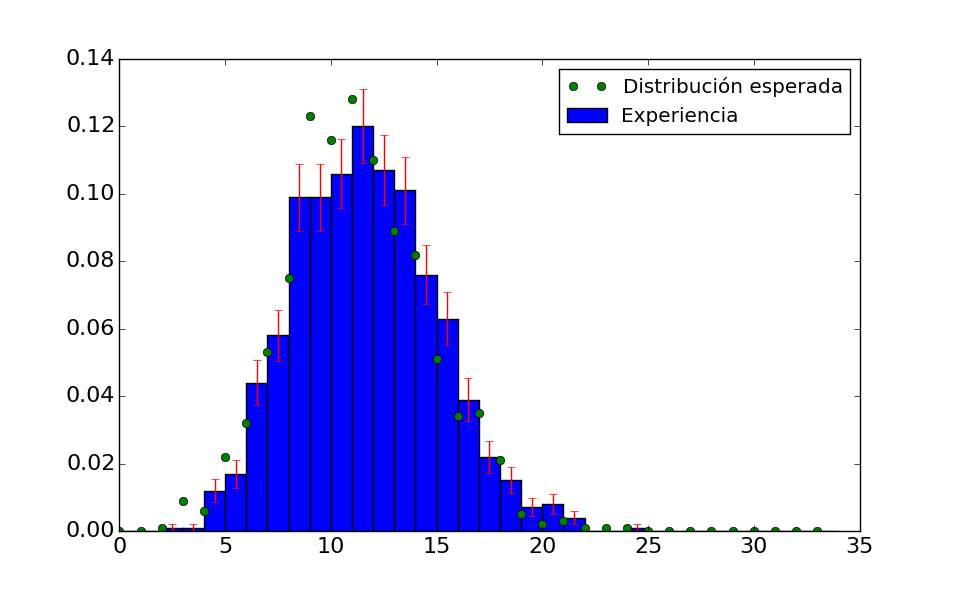
\includegraphics[width=0.45\textwidth]{proba_efectiva.png}
  \captionof{figure}{CAPTION}
  \label{fig:IMAGEN}
\end{center}

\section{Descripción de la experiencia}
\blindtext[14]

\newpage
\section{Resultados y discusión}
\Blindtext

\end{multicols}


\begin{center}
    \begin{tabular}{c c c c}
    \toprule
    Medición & Pendiente[mV$\,$mm$^{-1}$] & Ordenada[mV] & $\chi^2/dof$\\
    \midrule
    f = 1KHz y R = R$_{osc}$ & $(0,0565\pm0,0002$ & $(0,0121\pm0,0004)$ & 0,995\\
    f = 2,5KHz y R = R$_{osc}$ & $(0,0313\pm0,0001)$ & $(0,0299\pm0,0004)$ &0,998\\
    f = 5KHz y R = R$_{osc}$ &  $(0,0315\pm0,0003)$ & $(0.0058\pm0,0010)$ &0.984\\
    f = 2,5KHz y R = $(9,94\pm0,05)$K$\Omega$ &  $(0,0311\pm0,0004)$ & $(0,0051\pm0,0019)$ &0,991\\
    f = 5KHz y R = $(9,94\pm0,05)$K$\Omega$& $(0,0298\pm0,0005)$ & $(0,0044\pm0,0017)$ &0,862\\
    \bottomrule
    \end{tabular}
    \captionof{table}{DATOS}
    \label{tbl:DATOS}
\end{center}

\begin{multicols}{2}

\section{Conclusiones}
\blindtext[2]

\begin{thebibliography}{3}
  \bibitem{landau}
    Laundau, Lev D., Lifshitz, E. M., \emph{Mechanics}, vol. 1 de \emph{Course of theorical physics}, 3ed., 1986.
\end{thebibliography}

\end{multicols}

\newpage
\begin{multicols}{2}
\appendix
\section{Apéndice 1}
\blindtext
\section{Apéndice 2}
\blindtext
\end{multicols}


\end{document}
